
%%%%%%%%%%%%%%%%%%%%%%%%%%%%%%%%%%%%%%%%%%%%
\section{Les cosmologies antiques}

%%%%%%%%%%%%%%%%%%%%%%%%%%%%%%%%%%%%%%%%%%%%

  \subsection{Première cosmologie}

\begin{center}

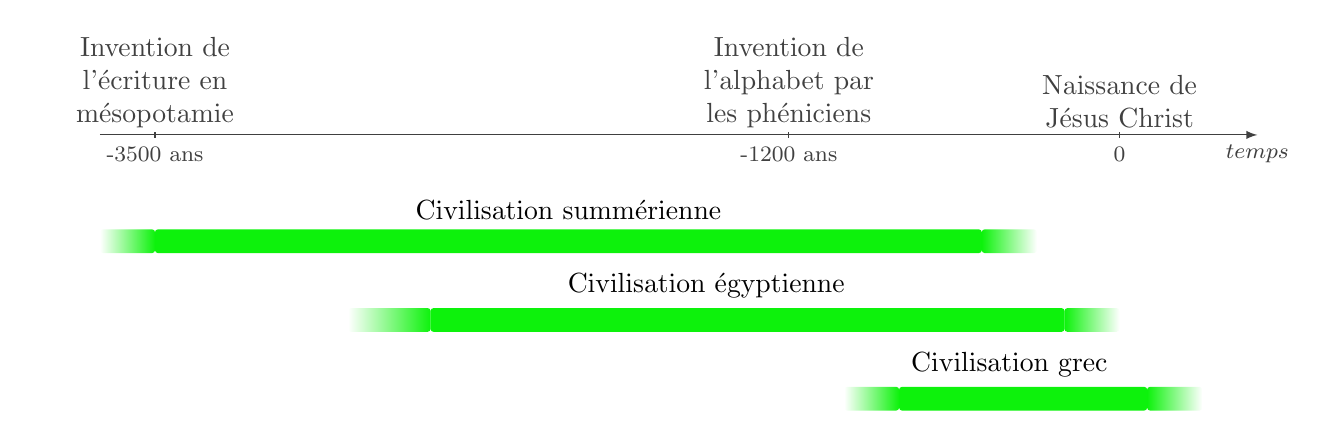
\begin{tikzpicture}
    \def\horizontal {0.35}
    \def\vertical {1.3}
\begin{scope}
\draw[-latex,color=darkgray] (-37*\horizontal,0) -- (5*\horizontal,0);
\draw[shift={(5*\horizontal,0)},color=darkgray,thin]
                                   node[below] {\footnotesize $temps$};
%3500 av JC
  \draw[shift={(-35*\horizontal,0)},color=darkgray,thin] (0pt,1pt) -- (0pt,-1pt)
                                   node[above,text width=3cm,text centered]{ Invention de l'écriture en mésopotamie}
                                   node[below] {\footnotesize -3500 ans};
%776 av JC
  \draw[shift={(-12*\horizontal,0)},color=darkgray,thin] (0pt,1pt) -- (0pt,-1pt)
                                   node[above,text width=3cm,text centered]{ Invention de l'alphabet par les phéniciens}
                                   node[below] {\footnotesize -1200 ans};
  \draw[shift={(0,0)},color=darkgray,thin] (0pt,1pt) -- (0pt,-1pt)
                                   node[below] {\footnotesize 0}
                                   node[above,text width=3cm,text centered]{ Naissance de Jésus Christ};
%\draw (1.4*\horizontal,0.5*\vertical) node [rotate=30]{Ptolémé};
\end{scope}
\begin{scope}[yshift= -1.5cm]
    \def\vertical {0.3}
  \shade[bottom color=brown!10!gray!10!green, top color=white,shading angle={90},rounded corners=1pt]
 (-37*\horizontal,0) rectangle (-35*\horizontal, \vertical);
  \shade[bottom color=brown!10!gray!10!green, top color=brown!10!gray!10!green,shading angle={90},rounded corners=1pt]
 (-35*\horizontal,0) rectangle (-5*\horizontal, \vertical);
  \shade[bottom color=white, top color=brown!10!gray!10!green,shading angle={90},rounded corners=1pt]
 (-5*\horizontal,0) rectangle (-3*\horizontal, \vertical);
  \node[above] (P) at (-20*\horizontal,\vertical) {Civilisation summérienne}; % SUMÉRIENS

    \def\decalage {-1}
  \shade[bottom color=brown!10!gray!10!green, top color=white,shading angle={90},rounded corners=1pt]
 (-28*\horizontal, \decalage) rectangle (-25*\horizontal, \vertical + \decalage);
  \shade[bottom color=brown!10!gray!10!green, top color=brown!10!gray!10!green,shading angle={90},rounded corners=1pt]
 (-25*\horizontal, \decalage) rectangle (-2*\horizontal, \vertical + \decalage);
  \shade[bottom color=white, top color=brown!10!gray!10!green,shading angle={90},rounded corners=1pt]
 (-2*\horizontal, \decalage) rectangle (0*\horizontal, \vertical + \decalage);
  \node[above] (P) at (-15*\horizontal,\vertical  + \decalage) {Civilisation égyptienne}; % ÉGYPTIENS

    \def\decalage {-2}
  \shade[bottom color=brown!10!gray!10!green, top color=white,shading angle={90},rounded corners=1pt]
 (-10*\horizontal, \decalage) rectangle (-8*\horizontal, \vertical + \decalage);
  \shade[bottom color=brown!10!gray!10!green, top color=brown!10!gray!10!green,shading angle={90},rounded corners=1pt]
 (-8*\horizontal, \decalage) rectangle (1*\horizontal, \vertical + \decalage);
  \shade[bottom color=white, top color=brown!10!gray!10!green,shading angle={90},rounded corners=1pt]
 (1*\horizontal, \decalage) rectangle (3*\horizontal, \vertical + \decalage);
  \node[above] (P) at (-4*\horizontal,\vertical  + \decalage) {Civilisation grec}; % CRECS
\end{scope}
\end{tikzpicture}


%%%%%%%%%%%%%%%%%%%%%%%%%%%%%%%%%%%%%%%%%%%




\end{center}

L'observation du ciel il y a des milliers d'années a conduit les hommes à se familiariser avec les phénomènes celeste.
 Le lien entre le mouvement des étoiles et le retour des saisons était utilisé pour l'agriculture.
 L'astronomie était alors surtout un outil de mesure du temps.

 Sont apparues alors des descriptions du monde en plus de la connaissances du mouvement des astres.
Ces descriptions sont les premiers modèles de cosmologie. Ils n'étaient pas accompagné d'explication rationnelle.

Les sumérien décrivaient l'univers comme une sphère et la Terre comme un disque entouré par la mer. 

\begin{center}


\begin{tikzpicture}
    \def\rayon {3}
    \def\vertical {1.3}

 %\shade[bottom color=blue!40!brown!40!, top color=cyan!20!]
 %\draw (0,0) circle (5cm);

\shade[bottom color=blue!10!cyan!10!, top color=blue!20!cyan!20!]
  (-\rayon,0) arc (180:0:\rayon) -- (-\rayon,0); % CIEL

\shade[bottom color=cyan!20!blue, top color=blue!60!cyan!20!]
  (-\rayon,0) arc (180:360:\rayon) -- (-\rayon,0); % MER

\shade[bottom color=cyan!10!blue!60!, top color=cyan!20!blue!60!]
 (0,0) ellipse (3 and 1.5); % MER

\shade[bottom color=green!20!brown!60!, top color=brown, decoration={random steps, segment length=0.1mm}, decorate]
 (0,0) ellipse (2 and 1); % TERRE
%\shade[bottom color=green!20!brown!40!, top color=green!40!brown!60!]
 %(0,0) ellipse (1.5 and 0.75);


%treetop/.style = {decoration={random steps, segment length=0.4mm}, decorate},1.4/40,1.2/50,1/60,

  \fill [green!60!black, decoration={random steps, segment length=0.4mm}, decorate](0,0) ellipse (1.6 and 0.8);
  \fill [green!40!black, decoration={random steps, segment length=0.4mm}, decorate](0.2,0) ellipse (0.8 and 0.4);
  \fill [green!70!black, decoration={random steps, segment length=0.4mm}, decorate](0,0.2) ellipse (0.6 and 0.3);
 % \fill [green!\f!black, decoration={random steps, segment length=0.4mm}, decorate](0,0) ellipse (\n *2 and \n);
 % \fill [green!\f!black, decoration={random steps, segment length=0.4mm}, decorate](0,0) ellipse (\n *2 and \n);


%\draw (-\rayon,0) arc (180:0:\rayon);



%(x0,y0) arc (angledébut:anglefin:rayon)

\end{tikzpicture}


%%%%%%%%%%%%%%%%%%%%%%%%%%%%%%%%%%%%%%%%%%%




\end{center}

Les égyptiens associaient le ciel et la Terre à des divinité et developpèrent une astrologie, croyance en un pouvoir des astres sur les hommes.

  \subsection{Les grecs}
Au premier millénaire avant notre ère, en Grèce, apparaît une volonté de rechercher une explication rationnelle du monde.
Les premières tentatives d'apporter cet ordre furent le fait de philosophes ioniens du {\footnotesize VII}$^\text{e}$ siècle avant J-C.

Apparurent alors plusieurs systèmes du monde différents. Ils décrivaient un {\it modèle} associé à des {\it principes naturelles} afin d'expliquer les observations, plutôt que de faire appel à la magie ou à la volonté des dieux. 

Au {\footnotesize VI}$^\text{e}$ siècle avant J-C, Pythagore et ses disciples développe une théorie du mouvement des corps célestes, appelée Harmonie des Sphères :

Des sphères en rotation portaient les corps célestes. La Terre était sphérique au centre du monde. La dernière sphère portait les étoiles fixes.


%Ce paradigme était incapable d'expliquer les irrégularités dans le déplacement des planètes, en particulier le mouvement rétrograde.
%%%%%%%%%%%%%%%%%%%%%%%%%%%%%%%%%%%%%%%%%%%



